\documentclass{beamer}
\usepackage[utf8]{inputenc}
\usepackage{graphicx, epsfig}
\usepackage{amsmath,mathrsfs,amsfonts,amssymb}
\usepackage{floatflt}
\usepackage{epic,ecltree}
\usepackage{mathtext}
\usepackage{fancybox}
\usepackage{fancyhdr}
\usepackage{multirow}
\usepackage{enumerate}
\usepackage{epstopdf}
\usepackage{multicol}
\usepackage{algorithm}
\usepackage[noend]{algorithmic}
\usepackage{tikz}
\usepackage{blindtext}
\usepackage{multido}
\usetheme{default}%{Singapore}%{Warsaw}%{Warsaw}%{Darmstadt}
\usecolortheme{default}

\setbeamerfont{title}{size=\Huge}
\setbeamertemplate{footline}[frame number]{}

\setbeamertemplate{section in toc}[sections numbered]

\makeatletter
\newcommand\HUGE{\@setfontsize\Huge{35}{40}}
\makeatother    

\setbeamerfont{title}{size=\HUGE}
\beamertemplatenavigationsymbolsempty

\usetikzlibrary{arrows,shapes,positioning,shadows,trees}

\newcommand\myfootnote[1]{%
  \vspace{-0.5cm}%
  \tikz[remember picture,overlay]
  \draw (current page.south west) +(1in + \oddsidemargin,0.5em)
  node[anchor=south west,inner sep=0pt]{\parbox{\textwidth}{%
      \rlap{\rule{10em}{0.4pt}}\raggedright\scriptsize \textit{#1}}};}

\newcommand\myfootnotewithlink[2]{%
  \vspace{-0.5cm}%
  \tikz[remember picture,overlay]
  \draw (current page.south west) +(1in + \oddsidemargin,0.5em)
  node[anchor=south west,inner sep=0pt]{\parbox{\textwidth}{%
      \rlap{\rule{10em}{0.4pt}}\raggedright\scriptsize\href{#1}{\textit{#2}}}};}

\AtBeginSection[]
      {
      	\begin{frame}{Outline}
      		\tableofcontents[currentsection]
      	\end{frame}
      }
      \AtBeginSubsection[]{
      	\begin{frame}{Outline}
      		\tableofcontents[currentsection,currentsubsection]
      	\end{frame}
}

\newcounter{noscounter}
\newcounter{pcounter}
\newcommand{\nextonslide}[1]{%
  \stepcounter{noscounter}%
  \stepcounter{pcounter}%
  \onslide<\value{noscounter}->{#1}%
}
\newcommand{\resetonslide}{%
    \setcounter{noscounter}{1}%
    \setcounter{pcounter}{0}%
}

\newcommand{\eqpause}{%
  \multido{\i=1+1}{\value{pcounter}}{\pause}%
  \stepcounter{noscounter}%
  \setcounter{pcounter}{0}%
  \pause%
}
\addtobeamertemplate{frametitle}{\resetonslide}{}

\input{../utils/newcommands}
\input{../utils/title}
\createdgmtitle{6}
%--------------------------------------------------------------------------------
\begin{document}
%--------------------------------------------------------------------------------
\begin{frame}[noframenumbering,plain]
%\thispagestyle{empty}
\titlepage
\end{frame}
%=======
\begin{frame}{Recap of previous lecture}
	\begin{block}{Assumptions}
		\begin{itemize}
			\item Let $c \sim \text{Categorical}(\bpi)$, where 
			\vspace{-0.6cm}
			\[
			\bpi = (\pi_1, \dots, \pi_K), \quad \pi_k = P(c = k), \quad \sum_{k=1}^K \pi_k = 1.
			\]
			\vspace{-0.7cm}
			\item Let the VAE model have a discrete latent representation $c$ with prior $p(c) = \text{Uniform}\{1, \dots, K\}$.
		\end{itemize}
	\end{block}
	\begin{block}{ELBO}
		\vspace{-0.6cm}
		\[
			\cL_{\bphi, \btheta}(\bx)  = \mathbb{E}_{q(c | \bx, \bphi)} \log p(\bx | c, \btheta) - {\color{olive} KL(q(c| \bx, \bphi) || p(c))} \rightarrow \max_{\bphi, \btheta}.
		\]
	\end{block}
	\vspace{-1.0cm}
	\[
		KL(q(c| \bx, \bphi) || p(c)) = - H(q(c | \bx, \bphi)) + \log K. 
	\]		
	\vspace{-0.5cm}
	\begin{block}{Vector Quantization}
		Define the dictionary space $\{\be_k\}_{k=1}^K$, where $\be_k \in \bbR^L$ and $K$ is the dictionary size.
		\vspace{-0.3cm}
		\[
		\bz_q = \bq (\bz) = \be_{k^*}, \quad \text{where } k^* = \argmin_k \| \bz - \be_k \|.
		\] 
		\vspace{-0.7cm}
	\end{block}
	\myfootnotewithlink{https://arxiv.org/abs/1711.00937}{Oord A., Vinyals O., Kavukcuoglu K. Neural Discrete Representation Learning, 2017} 
\end{frame}
%=======
\begin{frame}{Recap of previous lecture}
	\begin{figure}
		\centering
		\includegraphics[width=0.85\linewidth]{figs/vqvae}
	\end{figure}
	\vspace{-0.3cm}
	\begin{block}{Deterministic Variational Posterior}
		\vspace{-0.8cm}
		\[
			q(c_{ij} = k^* | \bx, \bphi) = \begin{cases}
				1 , \quad \text{for } k^* = \argmin_k \| [\bz_e]_{ij} - \be_k \|; \\
				0, \quad \text{otherwise}.
			\end{cases}
		\]
		\vspace{-0.8cm}
	\end{block}
	\begin{block}{ELBO}
		\vspace{-0.6cm}
		\[
			\cL_{\bphi, \btheta}(\bx)  = \mathbb{E}_{q(c | \bx, \bphi)} \log p(\bx | \be_{c} , \btheta) - \log K =  \log p(\bx | \bz_q, \btheta) - \log K.
		\]
		\vspace{-0.6cm}
	\end{block}
	\begin{block}{Straight-Through Gradient Estimation}
		\vspace{-0.6cm}
		\[
			\frac{\partial \log p(\bx | \bz_q , \btheta)}{\partial \bphi} = \frac{\partial \log p(\bx | \bz_q, \btheta)}{\partial \bz_q} \cdot {\color{red}\frac{\partial \bz_q}{\partial \bphi}} \approx \frac{\partial \log p(\bx | \bz_q, \btheta)}{\partial \bz_q} \cdot \frac{\partial \bz_e}{\partial \bphi}
		\]
	\end{block}
	\myfootnotewithlink{https://arxiv.org/abs/1711.00937}{Oord A., Vinyals O., Kavukcuoglu K. Neural Discrete Representation Learning, 2017} 
\end{frame}
%=======
\begin{frame}{Recap of previous lecture}
	\begin{block}{Theorem}
		\vspace{-0.6cm}
		\[
			\frac{1}{n} \sum_{i=1}^n KL(q(\bz | \bx_i, \bphi) || p(\bz)) = KL({\color{teal}q_{\text{agg}}(\bz | \bphi) }|| p(\bz)) + \bbI_{q} [\bx, \bz].
		\]
		\vspace{-0.6cm}
	\end{block}
	\begin{block}{ELBO Surgery}
		\vspace{-0.5cm}
		{\small
		\[
		    \frac{1}{n} \sum_{i=1}^n \cL_{\bphi, \btheta}(\bx_i) = \underbrace{\frac{1}{n} \sum_{i=1}^n \mathbb{E}_{q(\bz | \bx_i, \bphi)} \log p(\bx_i | \bz, \btheta)}_{\text{Reconstruction loss}}
		    - \underbrace{\vphantom{ \sum_{i=1}^n} \bbI_q [\bx, \bz]}_{\text{MI}} - \underbrace{\vphantom{ \sum_{i=1}^n} KL({\color{teal}q_{\text{agg}}(\bz | \bphi)} || {\color{violet}p(\bz)})}_{\text{Marginal KL}}
		\]}
	\end{block}
	\vspace{-0.7cm}
	\begin{block}{Optimal Prior}
		\vspace{-0.7cm}
		\[
			KL(q_{\text{agg}}(\bz | \bphi) || p(\bz)) = 0 \quad \Leftrightarrow \quad p (\bz) = q_{\text{agg}}(\bz) = \frac{1}{n} \sum_{i=1}^n q(\bz | \bx_i, \bphi).
		\]
		\vspace{-0.5cm}\\
		The optimal prior distribution $p(\bz)$ is the aggregated variational posterior $q_{\text{agg}}(\bz | \bphi)$.
	\end{block}
	\myfootnotewithlink{http://approximateinference.org/accepted/HoffmanJohnson2016.pdf}{Hoffman M. D., Johnson M. J. ELBO surgery: yet another way to carve up the variational evidence lower bound, 2016}
\end{frame}
%=======
\begin{frame}{Recap of previous lecture}
	\begin{itemize}
		\item Standard Gaussian $p(\bz) = \mathcal{N}(0, \bI)$ $\Rightarrow$ over-regularization;
		\item $p(\bz) = q_{\text{agg}}(\bz | \bphi) = \frac{1}{n}\sum_{i=1}^n q(\bz | \bx_i, \bphi)$ $\Rightarrow$ overfitting and extremely expensive.
	\end{itemize}
	\begin{block}{Revisiting ELBO}
		\vspace{-0.4cm}
		\[
		\frac{1}{n}\sum_{i=1}^n \cL_{\bphi, \btheta}(\bx_i) = \text{RL} - \text{MI} -  KL(q_{\text{agg}}(\bz | \bphi) || {\color{violet}p(\bz | \blambda)})
		\]
		It is the forward KL divergence with respect to $p(\bz | \blambda)$.
	\end{block}
	\begin{block}{ELBO with Learnable VAE Prior}
		\vspace{-0.6cm}
		{\small
			\begin{multline*}
				\cL_{\bphi, \btheta}(\bx) = \mathbb{E}_{q(\bz | \bx, \bphi)} \left[ \log p(\bx | \bz, \btheta) + {\color{violet}\log p(\bz | \blambda)} - \log q(\bz | \bx, \bphi) \right] \\
				= \mathbb{E}_{q(\bz | \bx, \bphi)} \Bigl[ \log p(\bx | \bz, \btheta) + \underbrace{ \Bigl({\color{violet} \log p(f_{\blambda}(\bz)) + \log \left| \det (\bJ_\bff) \right|} \Bigr) }_{\text{flow-based prior}} - \log q(\bz | \bx, \bphi) \Bigr] 
			\end{multline*}
		}
		\vspace{-0.5cm}
		\[
		\bz = \bff^{-1}_{\blambda}(\bz^*) = \bg_{\blambda}(\bz^*), \quad \bz^* \sim p(\bz^*) = \cN(0, \bI)
		\]
	\end{block}
	\vspace{-0.5cm}
	\myfootnotewithlink{https://arxiv.org/abs/1611.02731}{Chen X. et al. Variational Lossy Autoencoder, 2016}
\end{frame}
%=======
\begin{frame}{Outline}
	\tableofcontents
\end{frame}
%=======
\section{Likelihood-Free Learning}
%=======
\begin{frame}{Likelihood-Based Models}
	\begin{minipage}[t]{0.48\columnwidth}
		\begin{block}{Poor Likelihood \\ High-Quality Samples}
			\vspace{-0.3cm}
			\[
				p_1(\bx) = \frac{1}{n} \sum_{i=1}^n \cN(\bx | \bx_i, \epsilon \bI)
			\]
			If $\epsilon$ is small, this model generates high-quality samples, but the likelihood of a test sample will be very poor.
		\end{block}
	\end{minipage}%
	\begin{minipage}[t]{0.52\columnwidth}
		\begin{block}{High Likelihood \\ Poor Samples}
			\vspace{-0.5cm}
			\[
				p_2(\bx) = 0.01p(\bx) + 0.99p_{\text{noise}}(\bx)
			\]
			\vspace{-0.5cm}
			\begin{multline*}
				\log \left[ 0.01p(\bx) + 0.99p_{\text{noise}}(\bx) \right] \geq  \\ \geq \log \left[ 0.01p(\bx) \right]  = \log p(\bx) - \log 100
			\end{multline*}
			Contains mostly noisy, irrelevant samples, but for high dimensions $\log p(\bx)$ becomes proportional to $m$.
		\end{block}
	\end{minipage}
	\begin{itemize}
		\item Likelihood is not a perfect metric for evaluating generative models.
		\item The likelihood function may be intractable.
	\end{itemize}
	\myfootnotewithlink{https://arxiv.org/abs/1511.01844}{Theis L., Oord A., Bethge M. A note on the evaluation of generative models, 2015}
\end{frame}
%=======
\begin{frame}{Likelihood-Free Learning}
	\begin{block}{Motivation}
	 We aim to approximate the true data distribution $\pi(\bx)$.
	Instead of searching for the true $\pi(\bx)$ over all probability distributions, we learn a function $p(\bx | \btheta) \approx \pi(\bx)$.
	\end{block}
	Assume we have two sets of samples: 
	\begin{itemize}
		\item $\{\bx_i\}_{i=1}^{n_1} \sim \pi(\bx)$ — real samples;
		\item $\{\bx_i\}_{i=1}^{n_2} \sim p(\bx | \btheta)$ — generated (or fake) samples.
	\end{itemize}
	Define a discriminative model (classifier):
	\[
		p(y = 1 | \bx) = P\bigl(\bx \sim \pi(\bx)\bigr); \quad p(y = 0 | \bx) = P\bigl(\bx \sim p(\bx | \btheta)\bigr)
	\]
	\vspace{-0.5cm}
	\begin{block}{Assumption}
		The generative distribution $p(\bx | \btheta)$ matches the true distribution $\pi(\bx)$ if a discriminative model $p(y | \bx)$ cannot distinguish between them. \\
		This is equivalent to $p(y = 1 | \bx) = 0.5$ for every sample $\bx$.
	\end{block}

\end{frame}
%=======
\begin{frame}{Generative Adversarial Networks (GAN)}
	\begin{itemize}
		\item The more powerful the discriminative model, the more likely we are to obtain the optimal generative distribution $p(\bx | \btheta)$.
		\item The standard approach to learning a classifier is to minimize the cross-entropy loss.
	\end{itemize}
	\begin{block}{Cross-Entropy for Discriminative Model}
		\vspace{-0.3cm}
		\[
			\min_{p(y | \bx)} \left[ - \bbE_{\pi(\bx)} \log p(y = 1 | \bx) - \bbE_{p(\bx | \btheta)} \log p(y = 0 | \bx) \right] 
		\]
		\[
			\max_{p(y | \bx)} \left[\bbE_{\pi(\bx)} \log p(y = 1 | \bx) + \bbE_{p(\bx | \btheta)} \log p(y = 0 | \bx) \right] 
		\]
	\end{block}
	\vspace{-0.3cm}
	\begin{block}{Generative Model}
		Assume the generative model $p(\bx, \bz | \btheta) = p (\bx | \bz, \btheta) p(\bz)$, with a base distribution $p(\bz)$ and deterministic mapping $p (\bx | \bz, \btheta) = \delta (\bx - \bG_{\btheta}(\bz))$.
	\end{block}
	
	\myfootnotewithlink{https://arxiv.org/abs/1406.2661}{Goodfellow I. J. et al. Generative Adversarial Networks, 2014}
\end{frame}
%=======
\begin{frame}{Generative Adversarial Networks (GAN)}
	\begin{block}{Cross-Entropy for Discriminative Model}
		\vspace{-0.3cm}
		\[
			\max_{p(y | \bx)} \left[\bbE_{\pi(\bx)} \log p(y = 1 | \bx) + \bbE_{p(\bx | \btheta)} \log p(y = 0 | \bx) \right] 
		\]
	\end{block}
	\begin{itemize}
		\item \textbf{Discriminator:} a classifier $p(y = 1 | \bx, \bphi) = D_{\bphi}(\bx) \in [0, 1]$, distinguishing real samples from $\pi(\bx)$ and generated samples from $p(\bx | \btheta)$. The discriminator aims to \textbf{minimize} cross-entropy.
		\item \textbf{Generator:} the generative model $\bx = \bG_{\btheta}(\bz)$ where $\bz \sim p(\bz)$, seeking to make generated samples indistinguishable from real ones. The generator seeks to \textbf{maximize} cross-entropy.
	\end{itemize}
	\begin{block}{GAN Objective}
		\vspace{-0.5cm}
		\[
			\min_{G} \max_D \left[ \bbE_{\pi(\bx)} \log D(\bx) + \bbE_{p(\bx | \btheta)} \log (1 - D(\bx)) \right] 
		\]
		\[
			\min_{G} \max_D \left[ \bbE_{\pi(\bx)} \log D(\bx) + \bbE_{p(\bz)} \log (1 - D(\bG(\bz))) \right]
		\]
	\end{block}
	\myfootnotewithlink{https://arxiv.org/abs/1406.2661}{Goodfellow I. J. et al. Generative Adversarial Networks, 2014}
\end{frame}
%=======
\section{Generative Adversarial Networks (GAN)}
%=======
\begin{frame}{Generative Models Zoo}
	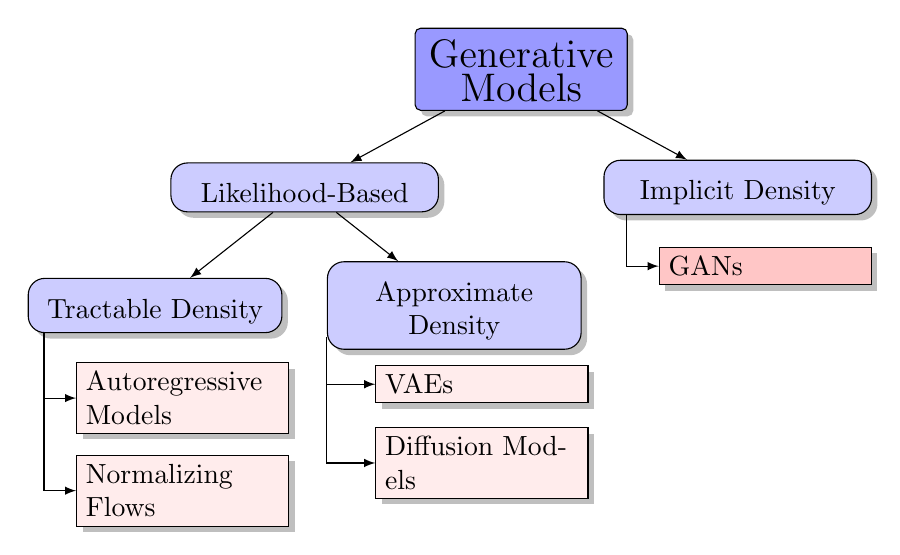
\begin{tikzpicture}[
	 	basic/.style  = {draw, text width=2cm, drop shadow, rectangle},
	 	root/.style   = {basic, rounded corners=2pt, thin, text height=1.1em, text width=7em, align=center, fill=blue!40},
	 	level 1/.style={sibling distance=55mm},
	 	level 2/.style = {basic, rounded corners=6pt, thin, align=center, fill=blue!20, text height=1.1em, text width=9em, sibling distance=38mm},
	 	level 3/.style = {basic, rounded corners=6pt, thin,align=center, fill=blue!20, text width=8.5em},
	 	level 4/.style = {basic, thin, align=left, fill=pink!30, text width=7em},
	 	level 5/.style = {basic, thin, align=left, fill=pink!90, text width=7em},
		edge from parent/.style={->,draw},
		>=latex]
		
		\node[root] {\Large Generative Models}
		child {node[level 2] (c1) {Likelihood-Based}
			child {node[level 3] (c11) {Tractable Density}}
			child {node[level 3] (c12) {Approximate Density}}
		}
		child {node[level 2] (c2) {Implicit Density}};
		
		\begin{scope}[every node/.style={level 4}]
		\node [below of = c11, yshift=-5pt, xshift=10pt] (c111) {Autoregressive Models};
		\node [below of = c111, yshift=-5pt] (c112) {Normalizing Flows};
		
		\node [below of = c12, xshift=10pt] (c121) {VAEs};
		\node [below of = c121] (c122) {Diffusion Models};
		\end{scope}
		
		\begin{scope}[every node/.style={level 5}]
		\node [below of = c2, xshift=10pt] (c21) {GANs};
		\end{scope}
		
		\foreach \value in {1,2}
		\draw[->] (c11.194) |- (c11\value.west);
		
		\foreach \value in {1,2}
		\draw[->] (c12.194) |- (c12\value.west);
		
		\draw[->] (c2.194) |- (c21.west);
		
	\end{tikzpicture}
\end{frame}
%=======
\begin{frame}{GAN Optimality}
	\begin{block}{Theorem}
		The following minimax game
		\vspace{-0.3cm}
		\[
			\min_{G} \max_D \Bigl[ \underbrace{\bbE_{\pi(\bx)} \log D(\bx) + \bbE_{p(\bz)} \log (1 - D(\bG(\bz)))}_{V(G, D)} \Bigr]
		\]
		\vspace{-0.5cm} \\
		attains its global optimum when $\pi(\bx) = p(\bx | \btheta)$, in which case $D^*(\bx) = 0.5$.
	\end{block}
	\begin{block}{Proof (Fixed $G$)}
		\vspace{-0.5cm}
		\begin{align*}
			V(G, D) &= \bbE_{\pi(\bx)} \log D(\bx) + \bbE_{p(\bx | \btheta)} \log (1 - D(\bx)) \\
			&= \int \underbrace{\left[ \pi(\bx) \log D(\bx) + p(\bx | \btheta)\log (1 - D(\bx)) \right]}_{y(D)} d \bx
		\end{align*}
		\vspace{-0.2cm}
		\[
			\frac{d y(D)}{d D} = \frac{\pi(\bx)}{D(\bx)} - \frac{p(\bx | \btheta)}{1 - D(\bx)} = 0 \quad \Rightarrow \quad D^*(\bx) = \frac{\pi(\bx)}{\pi(\bx) + p(\bx | \btheta)}
		\]
	\end{block}
	\myfootnotewithlink{https://arxiv.org/abs/1406.2661}{Goodfellow I. J. et al. Generative Adversarial Networks, 2014}
\end{frame}
%=======
\begin{frame}{GAN Optimality}
	\begin{block}{Proof Continued (Fixed $D = D^*$)}
		\vspace{-0.5cm}
		\begin{multline*}
			V(G, D^*) = \bbE_{\pi(\bx)} \log \left( \frac{\pi(\bx)}{\pi(\bx) + p(\bx | \btheta)} \right) + \bbE_{p(\bx | \btheta)} \log \left( \frac{p(\bx | \btheta)}{\pi(\bx) + p(\bx | \btheta)}\right)  \\
		 = KL \left(\pi(\bx) || \frac{\pi(\bx) + p(\bx | \btheta)}{2}\right) + KL \left(p(\bx | \btheta) || \frac{\pi(\bx) + p(\bx | \btheta)}{2}\right) - 2\log 2 \\
		 = 2JSD(\pi(\bx) || p(\bx | \btheta)) - 2\log 2.
		\end{multline*}
	\end{block}
	\vspace{-0.3cm}
	\begin{block}{Jensen-Shannon Divergence (Symmetric KL Divergence)}
		\vspace{-0.2cm}
		\footnotesize
		\[
			JSD(\pi(\bx) || p(\bx | \btheta)) = \frac{1}{2} \left[KL \left(\pi(\bx) || \frac{\pi(\bx) + p(\bx | \btheta)}{2}\right) + KL \left(p(\bx | \btheta) || \frac{\pi(\bx) + p(\bx | \btheta)}{2}\right) \right]
		\]
	\end{block}
	This can be used as a distance metric!
	\[
		V(G^*, D^*) = -2\log 2, \quad \pi(\bx) = p(\bx | \btheta), \quad  D^*(\bx) = 0.5.
	\]
	
	 \myfootnotewithlink{https://arxiv.org/abs/1406.2661}{Goodfellow I. J. et al. Generative Adversarial Networks, 2014}
\end{frame}
%=======
\begin{frame}{GAN Optimality}
	\begin{block}{Theorem}
		The following minimax game 
		\vspace{-0.3cm}
		\[
		\min_{G} \max_D \Bigl[ \bbE_{\pi(\bx)} \log D(\bx) + \bbE_{p(\bz)} \log (1 - D(\bG(\bz))) \Bigr]
		\]
		\vspace{-0.5cm} \\
		attains its global optimum when $\pi(\bx) = p(\bx | \btheta)$, in which case $D^*(\bx) = 0.5$.
	\end{block}
	\vspace{-0.2cm}
	\begin{block}{Expectations}
		If the generator can be \textbf{any} function and the discriminator is \textbf{optimal} at every step, then the generator is \textbf{guaranteed to converge} to the data distribution.
	\end{block}
	\begin{block}{Reality}
		\begin{itemize}
			\item Generator updates are made in parameter space, the discriminator is not always optimal.
			\item The generator and discriminator losses typically oscillate during GAN training.
		\end{itemize}
	\end{block}
	 \myfootnotewithlink{https://arxiv.org/abs/1406.2661}{Goodfellow I. J. et al. Generative Adversarial Networks, 2014}
\end{frame}
%=======
\begin{frame}{GAN Training}
	Assume the generator and discriminator are parametric models: $D_{\bphi}(\bx)$ and $\bG_{\btheta}(\bz)$.
	\begin{block}{Objective}
		\vspace{-0.7cm}
		\[
		\min_{\btheta} \max_{\bphi} \left[ \bbE_{\pi(\bx)} \log D_{\bphi}(\bx) + \bbE_{p(\bz)} \log (1 - D_{\bphi}(\bG_{\btheta}(\bz))) \right]
		\]
		\vspace{-0.7cm}
	\end{block}
	\begin{figure}
		\centering
		\includegraphics[width=1.0\linewidth]{figs/gan_1}
	\end{figure}

	\begin{itemize}
		\item $\bz \sim p(\bz)$ is a latent variable.
		\item $p(\bx | \bz, \btheta) = \delta(\bx - \bG_{\btheta}(\bz))$ is a deterministic decoder ({\color{gray} like NF}).
		\item There is no encoder at all.
	\end{itemize}

	 \myfootnotewithlink{https://arxiv.org/abs/1406.2661}{Goodfellow I. J. et al. Generative Adversarial Networks, 2014}
\end{frame}
%=======
\begin{frame}{Mode Collapse}
	Mode collapse refers to the phenomenon where the generator in a GAN collapses to just one or a few modes of the distribution.
	\vspace{-0.15cm}
	\begin{figure}
		\centering
		\includegraphics[width=0.75\linewidth]{figs/mode_collapse_1}
	\end{figure}
	\vspace{-0.3cm}
	\begin{figure}
		\centering
		\includegraphics[width=1.0\linewidth]{figs/mode_collapse_4}
	\end{figure}
	Alternative architectures, additional regularization terms, the injection of small noise perturbations, and numerous other tricks have been used to address mode collapse.
	
	\myfootnote{\href{https://arxiv.org/abs/1406.2661}{Goodfellow I. J. et al. Generative Adversarial Networks, 2014} \\
		\href{https://arxiv.org/abs/1611.02163}{Metz L. et al. Unrolled Generative Adversarial Networks, 2016}}
\end{frame}
%=======
\begin{frame}{Jensen-Shannon vs Kullback-Leibler divergences}
	\begin{itemize}
		\item $\pi(\bx)$ is a fixed mixture of 2 Gaussians.
		\item $p(\bx | \mu, \sigma) = \cN(\mu, \sigma^2)$.
	\end{itemize}
	\begin{block}{Mode Covering vs. Mode Seeking}
		\vspace{-0.7cm}
		\[
		KL(\pi || p) = \int \pi(\bx) \log \frac{\pi(\bx)}{p(\bx)}d\bx, \quad KL(p || \pi) = \int p(\bx) \log \frac{p(\bx)}{\pi(\bx)}d\bx
		\]
		\[
		JSD(\pi || p) = \frac{1}{2} \left[KL \left(\pi(\bx) || \frac{\pi(\bx) + p(\bx)}{2}\right) + KL \left(p(\bx) || \frac{\pi(\bx) + p(\bx)}{2}\right) \right]
		\]
		\vspace{-0.7cm}
		
		\begin{minipage}[t]{0.33\columnwidth}
			\begin{figure}
				\includegraphics[width=\linewidth]{figs/forward_KL}
			\end{figure}
		\end{minipage}%
		\begin{minipage}[t]{0.33\columnwidth}
			\begin{figure}
				\includegraphics[width=\linewidth]{figs/reverse_KL}
			\end{figure}
		\end{minipage}%
		\begin{minipage}[t]{0.33\columnwidth}
			\begin{figure}
				\includegraphics[width=\linewidth]{figs/JSD}
			\end{figure}
		\end{minipage}
		\vspace{-0.3cm}
	\end{block}
\end{frame}
%=======
\section{Wasserstein Distance}
%=======
\begin{frame}{al Theoretical Results}
	\vspace{-0.3cm}
	\begin{itemize}
		\item The dimensionality of $\bz$ is less than that of $\bx$. Thus, the support of $p(\bx | \btheta)$ with $\bx = \bG_{\btheta}(\bz)$ lies on a low-dimensional manifold.
		\item The distribution of real images $\pi(\bx)$ is also concentrated on a low-dimensional manifold.
		\begin{figure}
			\centering
			\includegraphics[width=0.55\linewidth]{figs/low_dim_manifold}
		\end{figure}
		\item If $\pi(\bx)$ and $p(\bx | \btheta)$ have disjoint supports, then a smooth optimal discriminator exists.
		\item For such low-dimensional, disjoint manifolds:
		\vspace{-0.2cm}
		\[
		KL(\pi || p) = KL(p || \pi) = \infty, \quad JSD(\pi || p) = \log 2
		\]
	\end{itemize}
	\myfootnote{\href{https://arxiv.org/abs/1904.08994}{Weng L. From GAN to WGAN, 2019} \\ 
		\href{https://arxiv.org/abs/1701.04862}{Arjovsky M., Bottou L. Towards Principled Methods for Training Generative Adversarial Networks, 2017}}
\end{frame}
%=======
\begin{frame}{Wasserstein Distance (Discrete)}
	Also known as \textbf{Earth Mover's Distance}.
	\begin{block}{Optimal Transport Formulation}
		The minimum cost of moving and transforming a pile of "dirt" from the shape of one probability distribution into the shape of another.
	\end{block}
	\begin{figure}
		\centering
		\includegraphics[width=\linewidth]{figs/discrete_wasserstein}
	\end{figure}
	\myfootnotewithlink{https://udlbook.github.io/udlbook/}{Simon J.D. Prince. Understanding Deep Learning, 2023}
\end{frame}
%=======
\begin{frame}{Wasserstein Distance (Continuous)}
	\vspace{-0.7cm}
	\[
	W(\pi, p) = \inf_{\gamma \in \Gamma(\pi, p)} \bbE_{(\bx, \by) \sim \gamma} \| \bx - \by \| =  \inf_{{\color{olive}\gamma}\in {\color{teal}\Gamma(\pi, p)}} \int {\color{violet} \| \bx - \by \|} {\color{olive}\gamma (\bx, \by)} d \bx d \by
	\]
	\vspace{-0.4cm}
	\begin{itemize}
		\item ${\color{olive}\gamma (\bx, \by)}$: the transportation plan (i.e., the amount of "dirt" transported from $\bx$ to $\by$).
		\vspace{-0.2cm}
		\[
		\int \gamma(\bx, \by) d \bx = p(\by); \quad \int \gamma(\bx, \by) d \by = \pi(\bx).
		\]
		\vspace{-0.6cm}
		\item ${\color{teal}\Gamma(\pi, p)}$ denotes the set of all joint distributions $\gamma (\bx, \by)$ with marginals $\pi$ and $p$.
		\item ${\color{olive}\gamma(\bx, \by)}$ is the amount, ${\color{violet} \| \bx - \by \|}$ is the distance.
	\end{itemize}
	\begin{block}{Wasserstein Metric}
		\vspace{-0.2cm}
		\[
		W_s(\pi, p) = \inf_{\gamma \in \Gamma(\pi, p)} \left(\bbE_{(\bx, \by) \sim \gamma} \| \bx - \by \|^s\right)^{1/s}
		\]
		\vspace{-0.4cm}
	\end{block}
	In this context, we use $W(\pi, p) = W_1(\pi, p)$, corresponding to the optimal transport formulation.
	\myfootnotewithlink{https://arxiv.org/abs/1701.07875}{Arjovsky M., Chintala S., Bottou L. Wasserstein GAN, 2017}
\end{frame}
%=======
\begin{frame}{Wasserstein Distance vs KL vs JSD}
	
	\begin{minipage}[t]{0.48\columnwidth}
		\vspace{0.1cm}
		Consider two-dimensional distributions:
		\[
		\pi(x, y) = (0, U[0,1])
		\]	
		\[
		p(x, y | \theta) = (\theta, U[0, 1])
		\]
	\end{minipage}%
	\begin{minipage}[t]{0.52\columnwidth}
		\begin{figure}
			\centering
			\includegraphics[width=0.8\linewidth]{figs/w_kl_jsd}
		\end{figure}
	\end{minipage}
	\begin{itemize}
		\footnotesize
		\item $\theta = 0$.
		Distributions are identical:
		\[
		KL(\pi || p) = KL(p || \pi) = JSD(p || \pi) = W(\pi, p) = 0
		\]
		\item $\theta \neq 0$
		\[
		KL(\pi || p) = \int_{U[0, 1]} 1 \log \frac{1}{0} d y = \infty = KL(p || \pi)
		\]
		\[
		JSD(\pi || p) = \frac{1}{2}\left( \int_{U[0, 1]}1 \log \frac{1}{1/2} dy + \int_{U[0, 1]}1 \log \frac{1}{1/2} dy \right) = \log 2
		\]
		\[
		W(\pi, p) = |\theta|
		\]
	\end{itemize}
	
	\myfootnote{\href{https://arxiv.org/abs/1904.08994}{Weng L. From GAN to WGAN, 2019} \\ 
		\href{https://arxiv.org/abs/1701.07875}{Arjovsky M., Chintala S., Bottou L. Wasserstein GAN, 2017}}
\end{frame}
%=======
\begin{frame}{Wasserstein Distance vs KL vs JSD}
	\begin{block}{Theorem 1}
		Let $\bG_{\btheta}(\bz)$ be (almost) any feedforward neural network, and $p(\bz)$ a prior over $\bz$ such that $\bbE_{p(\bz)} \|\bz\| < \infty$. Then $W(\pi, p)$ is continuous everywhere and differentiable almost everywhere.
	\end{block}
	\begin{block}{Theorem 2}
		Let $\pi$ be a distribution on a compact space $\cX$ and let $\{p_t\}_{t=1}^\infty$ be a sequence of distributions on $\cX$. 
		\begin{align}
			KL(\pi || p_t) &\rightarrow 0 \ \ (\text{or }KL (p_t || \pi) \rightarrow 0) \\
			JSD(\pi || p_t) &\rightarrow 0 \\
			W(\pi || p_t) &\rightarrow 0
		\end{align}
		
		In other words, as $t \rightarrow \infty$, (1) implies (2), and (2) implies (3).
	\end{block}
	\myfootnotewithlink{https://arxiv.org/abs/1701.07875}{Arjovsky M., Chintala S., Bottou L. Wasserstein GAN, 2017}
\end{frame}
%=======
\section{Wasserstein GAN}
%=======
\begin{frame}{Wasserstein GAN}
	\begin{block}{Wasserstein Distance}
		\vspace{-0.5cm}
		\[
		W(\pi || p) = \inf_{\gamma \in \Gamma(\pi, p)} \bbE_{(\bx, \by) \sim \gamma} \| \bx - \by \| =  \inf_{\gamma \in \Gamma(\pi, p)} \int \| \bx - \by \| \gamma (\bx, \by) d \bx d \by
		\]
		\vspace{-0.3cm}
	\end{block}
	The infimum over all possible joint distributions in $\Gamma(\pi, p)$ is intractable.
	\begin{block}{Theorem (Kantorovich-Rubinstein Duality)}
		\vspace{-0.3cm}
		\[
		W(\pi || p) = \frac{1}{K} \max_{\| f \|_L \leq K} \left[ \bbE_{\pi(\bx)} f(\bx)  - \bbE_{p(\bx)} f(\bx)\right],
		\]
		where $f : \bbR^m \rightarrow \bbR$, $\| f \|_L \leq K$ are $K$-Lipschitz continuous functions ($f: \cX \rightarrow \bbR$)
		\vspace{-0.2cm}
		\[
		|f(\bx_1) - f(\bx_2)| \leq K \| \bx_1 - \bx_2 \|, \quad \forall \bx_1, \bx_2 \in \cX.
		\]
		\vspace{-0.6cm}
	\end{block}
	Now we can use just samples to compute a Monte Carlo estimate for $W(\pi || p)$.
	
	\myfootnotewithlink{https://arxiv.org/abs/1701.07875}{Arjovsky M., Chintala S., Bottou L. Wasserstein GAN, 2017}
\end{frame}
%=======
\begin{frame}{Wasserstein GAN}
	\begin{block}{Theorem (Kantorovich-Rubinstein Duality)}
		\[
		W(\pi || p) = \frac{1}{K} \max_{\| f \|_L \leq K} \left[ \bbE_{\pi(\bx)} f(\bx)  - \bbE_{p(\bx)} f(\bx)\right],
		\]
	\end{block}
	\begin{itemize}
		\item We must ensure that $f$ is $K$-Lipschitz continuous.
		\item Let $f_{\bphi}(\bx)$ be a feedforward neural network parametrized by $\bphi$.
		\item If the parameters $\bphi$ lie in a compact set $\boldsymbol{\Phi}$, then $f_{\bphi}(\bx)$ is $K$-Lipschitz continuous.
		\item Clamp the parameters to a fixed box $\boldsymbol{\Phi} \in [-c, c]^d$ (e.g., $c = 0.01$) after each gradient update.
	\end{itemize}
	\begin{multline*}
		K \cdot W(\pi || p) = \max_{\| f \|_L \leq K} \left[ \bbE_{\pi(\bx)} f(\bx)  - \bbE_{p(\bx)} f(\bx)\right] \geq \\  \geq \max_{\bphi \in \boldsymbol{\Phi}} \left[ \bbE_{\pi(\bx)} f_{\bphi}(\bx)  - \bbE_{p(\bx)} f_{\bphi}(\bx)\right]
	\end{multline*}
	
	\myfootnotewithlink{https://arxiv.org/abs/1701.07875}{Arjovsky M., Chintala S., Bottou L. Wasserstein GAN, 2017}
\end{frame}
%=======
\begin{frame}{Wasserstein GAN}
	\begin{block}{Standard GAN Objective}
		\vspace{-0.2cm}
		\[
		\min_{\btheta} \max_{\bphi} \bbE_{\pi(\bx)} \log D_{\bphi}(\bx) + \bbE_{p(\bz)} \log (1 - D_{\bphi}(\bG_{\btheta}(\bz)))
		\]
		\vspace{-0.3cm}
	\end{block}
	\begin{block}{WGAN Objective}
		\vspace{-0.3cm}
		\[
		\min_{\btheta} {\color{violet}W(\pi || p)} \approx \min_{\btheta} {\color{violet}\max_{\bphi \in \boldsymbol{\Phi}} \left[ \bbE_{\pi(\bx)} f_{\bphi}(\bx)  - \bbE_{p(\bz)} f_{\bphi}(\bG_{\btheta}(\bz))\right]}.
		\]
		\vspace{-0.3cm}
	\end{block}
	\begin{itemize}
		\item The discriminator $D$ is analogous to the function $f$ but is not a classifier anymore. In WGAN, $f$ is typically termed the \textbf{critic}.
		\item \textit{"Weight clipping is a clearly terrible way to enforce a Lipschitz constraint."} 
		\begin{itemize}
			\item If the clipping parameter $c$ is too large, it is difficult to train the critic to optimality.
			\item If $c$ is too small, it can lead to vanishing gradients.
		\end{itemize}
	\end{itemize}
	
	\myfootnotewithlink{https://arxiv.org/abs/1701.07875}{Arjovsky M., Chintala S., Bottou L. Wasserstein GAN, 2017}
\end{frame}
%=======
\begin{frame}{Wasserstein GAN}
	\begin{minipage}[t]{0.6\columnwidth}
		\begin{itemize}
			\item WGAN yields non-zero gradients even for distributions with disjoint supports.
			\item $JSD(\pi || p)$ is poorly correlated with sample quality and stays nearly constant at its maximum value $\log 2 \approx 0.69$.
			\item $W(\pi || p)$ is highly correlated with sample quality. 
		\end{itemize}
	\end{minipage}%
	\begin{minipage}[t]{0.4\columnwidth}
		\begin{figure}
			\centering
			\includegraphics[width=\linewidth]{figs/wgan_toy}
		\end{figure}
	\end{minipage}
	\begin{minipage}[t]{0.5\columnwidth}
		\begin{figure}
			\centering
			\includegraphics[width=1.0\linewidth]{figs/dcgan_quality}
		\end{figure}
	\end{minipage}%
	\begin{minipage}[t]{0.5\columnwidth}
		\begin{figure}
			\centering
			\includegraphics[width=1.0\linewidth]{figs/wgan_quality}
		\end{figure}
	\end{minipage}
	\myfootnotewithlink{https://arxiv.org/abs/1701.07875}{Arjovsky M., Chintala S., Bottou L. Wasserstein GAN, 2017}
\end{frame}
%=======
\begin{frame}{Summary}
	\begin{itemize}
		\item Likelihood is not a reliable criterion for assessing the quality of generative models.		
		\vfill
		\item Adversarial learning proposes solving a minimax problem to match distributions.
		\vfill
		\item GANs aim to optimize the Jensen-Shannon divergence (in theory).
		\vfill
		\item KL and JS divergences are unsuitable objectives when the supports of the distributions are disjoint.
		\vfill
		\item The Earth Mover's distance provides a more appropriate objective for distribution matching.
		\vfill
		\item The Kantorovich-Rubinstein duality provides a way to compute the EM distance using only samples.
		\vfill
		\item Wasserstein GAN enforces the Lipschitz constraint on the critic via weight clipping.
	\end{itemize}
\end{frame}

\end{document}
